\chapter{History-dependent variability in population dynamics during evidence accumulation in cortex} \label{chapter_3}

\vspace*{-44pt}

Ari S. Morcos and Christopher D. Harvey

\smallskip
\textit{This and the following chapters are a modified version of a submitted manuscript.}

\vspace*{50pt}

\section{Introduction} \label{sec:chap3_intro}

The activity patterns in a cortical microcircuit are determined both by the characteristics of the external inputs it receives and the dynamic, ongoing changes in its internal activity state. The computation to combine ongoing activity with new inputs is essential for many complex behaviors, including evidence accumulation during decision-making. Much work has focused on identifying the neuronal algorithms and mechanisms by which evidence accumulation occurs, with considerable emphasis on the posterior parietal cortex (PPC) \citep{Shadlen:1996ga, Gold:2000hp, Yang:2007in, Hanks:2015fy, Britten:1992wx}. Previous work has modeled evidence accumulation as a competition between distinct pools of neurons with recurrent excitation within a pool and mutual inhibition across pools \citep{Wong:2006in, Wang:2002kn}. The activity of individual neurons in these models is long-lasting within a trial and homogeneous across neurons. These models propose a ‘winner-take-all’ competition between these neuronal groups in which activity eventually converges to one of several attractor states \citep{Wong:2006in, Machens:2005en, Wang:2002kn}. Although such models are consistent with some experimental results \citep{Shadlen:1996ga, Gold:2000hp, Yang:2007in, Hanks:2015fy, Britten:1992wx, Horwitz:1999ws}, our recent work in the mouse PPC during a navigation-based decision task found that neurons had transient, time-varying activity that was heterogeneous across neurons \citep{Harvey:2012du}. These results led us to conceptualize the activity in the PPC on single trials as a trajectory of time-varying neuronal population activity patterns. The apparent inconsistencies between our previous results and traditional models revealed to us the lack of competing algorithmic models for evidence accumulation. 

\bigskip
Here, we used the conceptual framework of time-varying neuronal population activity trajectories to study neuronal population dynamics on single trials during evidence accumulation. Previous work has emphasized independent recordings from selected subsets of individual neurons, summarized as averages across trials and cells, in part because of technical challenges in measuring and interpreting neuronal population activity on single trials. We therefore developed new experimental and computational methods based on unbiased sampling of activity from large populations of neurons to reveal structure in the moment-to-moment changes in population activity.

\bigskip
We found that the PPC had long timescale dynamics in the form of structured transitions between transient and largely uncorrelated patterns of population activity. New inputs to the network, including evidence cues and behavioral choices, constrained the possible population activity patterns for seconds into the future. This effect occurred by changing the transition probabilities between activity patterns consisting of largely different combinations of active neurons. The population-level representation of new inputs thus depended both on the identity of the input and the near-past activity patterns in the population, such that PPC activity never reset but rather functioned as a continuous record of recent events. In addition, multiple task-relevant features were represented simultaneously, distributed across populations of heterogeneous and variable neurons, such that single task features (e.g., choice) did not converge to single activity patterns but rather were represented across trials by many different activity patterns. These results are inconsistent with evidence accumulation models that require a direct competition between two or more groups of neurons \citep{Wong:2006in, Machens:2005en, Wang:2002kn}, and instead reveal novel features of PPC dynamics that motivate a new algorithmic model based on general purpose, history-dependent dynamics.



\begin{figure}
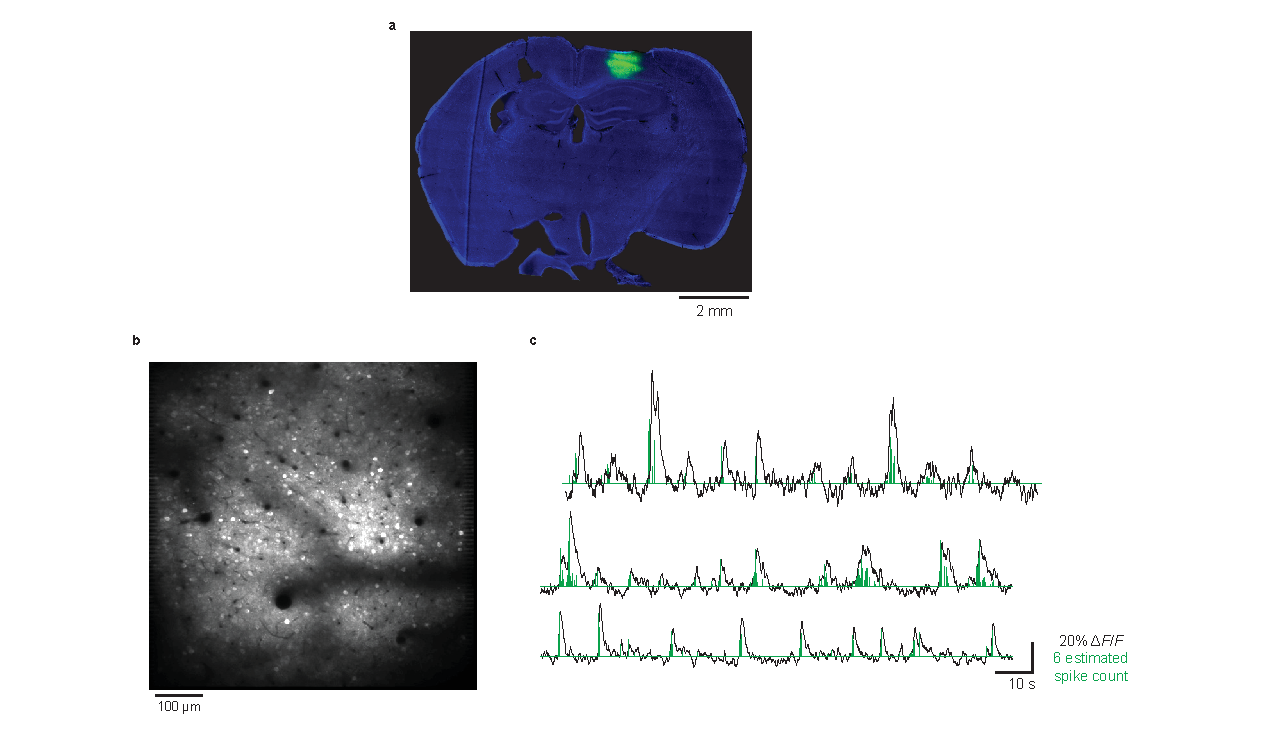
\includegraphics[width=1.1\textwidth,center]{figures/fig_3_1.pdf}
\caption[Example imaging field of view and activity traces.]{\textbf{Example imaging field of view and activity traces. a,} Example histology image of GCaMP6m-expressing neurons in the PPC. 
%
\textbf{b,} Example two-photon image of GCaMP6m-expressing neurons in layer 2/3 of the PPC. 
%
\textbf{c,} Example $\Delta$F/F traces (black) and deconvolved estimated spike counts (green) (Methods \ref{methods:preprocessing}).
\label{fig:3_1}}
\end{figure}

\begin{figure}
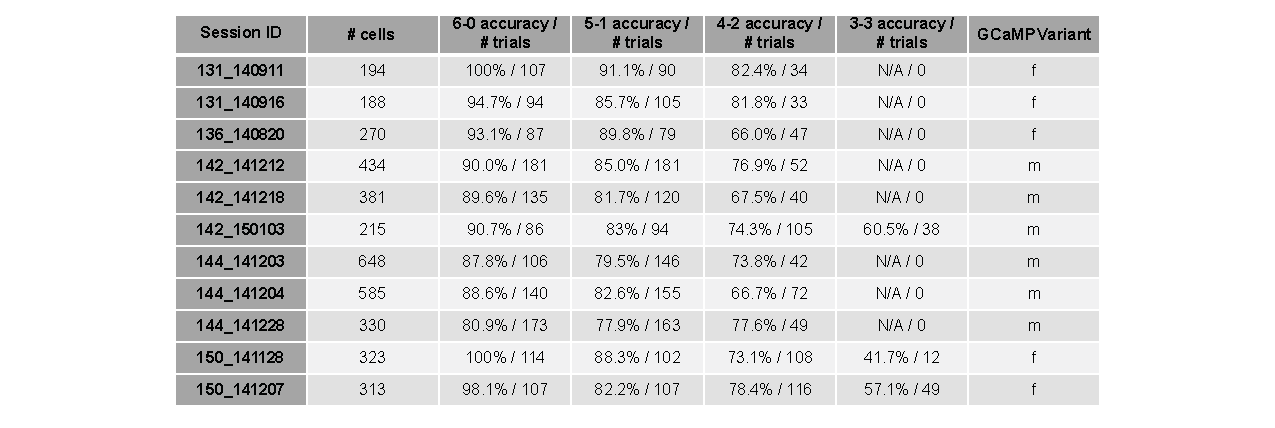
\includegraphics[width=1.5\textwidth,center]{figures/fig_3_2.pdf}
\caption[Summary of datasets analyzed.]{\textbf{Summary of datasets analyzed.}
\label{fig:3_2}}
\end{figure}

\section{Results} \label{sec:chap3_results}

We used the fixed association evidence accumulation task described in Section \ref{sec:fixed_section}. Briefly, as mice ran down a virtual T-maze, they were presented with six visual cues that could each appear on the left or the right wall at fixed locations (Figures \ref{fig:2_2}a-b, \ref{fig:2_3}). To receive a reward, the mouse had to turn at the T-intersection toward the direction that had more cues. Mice performed the task with high accuracy by accumulating multiple pieces of evidence, with a bias towards early cues (Figures \ref{fig:2_2}c, \ref{fig:2_4}).

\subsection{Single neuron responses during evidence accumulation} \label{sec:chap3_single_neuron}

We began our analysis of neuronal population activity during this task by examining the distribution of activity patterns in individual neurons. We used calcium imaging to measure the activity of 350 neurons simultaneously in layer 2/3 of the PPC and extracted estimated spike counts using deconvolution of the fluorescence traces \citep{Vogelstein:2010jl} (Methods \ref{methods:imaging}; Figures \ref{fig:3_1}, \ref{fig:3_2}). Consistent with our previous work, most neurons were transiently active for less than 10\% of the trial on average, and different neurons were active at different points in the trial, such that across the population, activity tiled the full trial duration \citep{Harvey:2012du} (Figures \ref{fig:3_3}a, \ref{fig:3_4}, \ref{fig:3_5}a-b). To test for differences in activity between trials with different choices and net evidence, we calculated a selectivity index for choice and used a support vector regression (SVR) model to predict net evidence from a single cell’s activity (Methods \ref{methods:choice_sel}, \ref{methods:multi_class_classifications}). A fraction of neurons had a statistically significant choice selectivity index, and some neurons had a significant relationship between the actual net evidence and the net evidence predicted from their activity (choice 20.2\%, net evidence 22.7\%; 5\% expected by chance; Figure \ref{fig:3_3}c-d). When we plotted the mean activity patterns for the neurons with choice selectivity, we identified choice-specific sequences of activity, consistent with PPC activity patterns during less complex decision tasks \citep{Harvey:2012du} (Figure \ref{fig:3_4}c-d). However, the majority of neurons did not have significantly different activity between trials of different choices and net evidence, consistent with our previous results \citep{Harvey:2012du}. The distribution of choice selectivity indices and net evidence prediction accuracies for single neurons largely overlapped with the distribution from shuffled data (Figure \ref{fig:3_3}c-d). The low selectivity values in these neurons resulted from unreliable responses with varying activity times between trials of the same type and similar activity between trials of different types. 

\subsection{Task-relevant information is distributed across neuronal populations} \label{sec:chap3_distributed}

Although the majority of individual neurons lacked strong selectivity, the population activity (concatenated activity of all individual neurons) contained information about the choice and net evidence on single trials with high accuracy. We quantified this selectivity using a support vector machine (SVM) classifier for choice and a SVR model to compare actual net evidence with the net evidence predicted by the population activity (Figure \ref{fig:3_3}e-f). 

\begin{FPfigure}
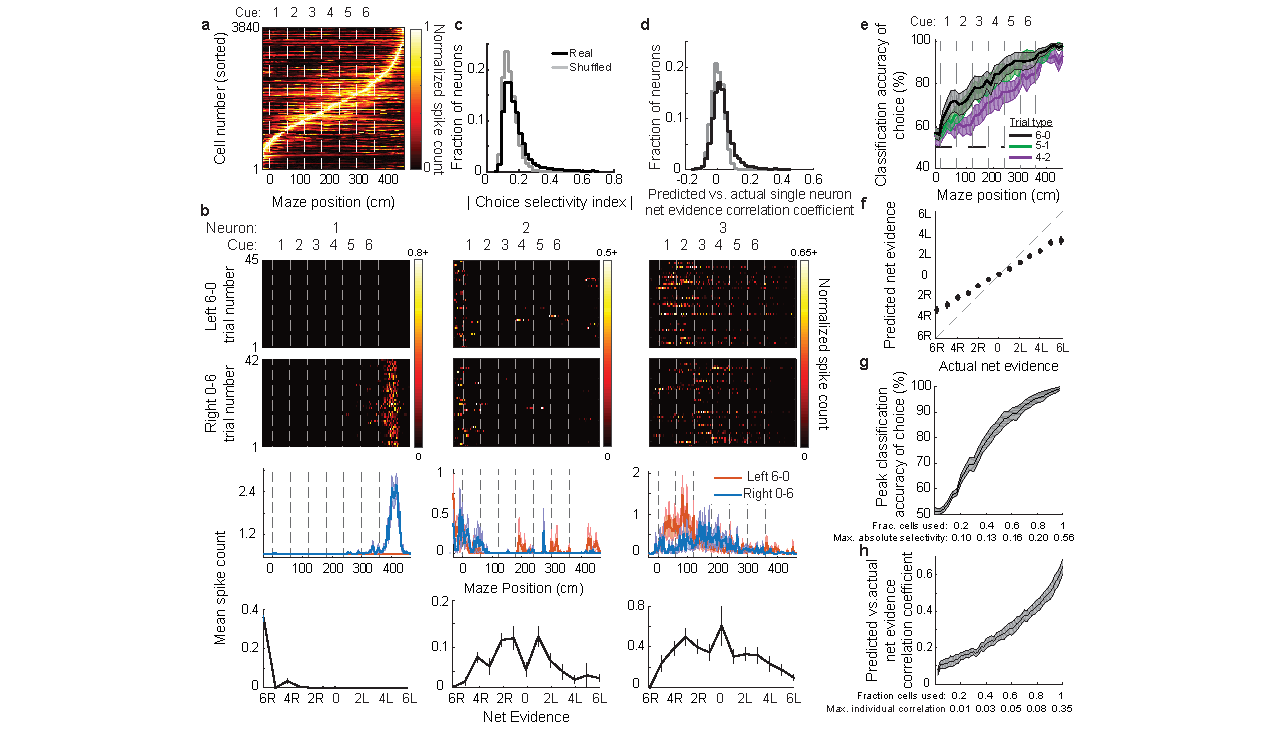
\includegraphics[width=1.5\textwidth,center]{figures/fig_3_3.pdf}
\caption[Distributed representation of task-relevant information across PPC neurons.]
{\textbf{Distributed representation of task-relevant information across PPC neurons. a,} Normalized mean activity across all trials for all neurons pooled across all datasets (n = 3840 cells from 5 mice). Traces were normalized to the peak of each cell's activity, averaged, and sorted by the peak's maze position. 
%
\textbf{b,} Single trial activity on left 6-0 and right 0-6 trials for three example neurons. Top panels: each row is an individual trial. Bottom panels: mean $\pm$ s.e.m. For each net evidence condition (e.g., 2L), the mean spike count was calculated by combining the activity at all cue epochs matching the given net evidence. 
%
\textbf{c,} Histogram of the the choice selectivity index for individual neurons (black) and with shuffled trial labels (gray). Choice selectivity was calculated separately for each spatial bin, and the maximum magnitude across bins was taken for each neuron. Choice selectivity for each neuron was calculated based on activity in left 6-0 and right 0-6 trials (Methods \ref{methods:choice_sel}).
%
\textbf{d,} Histogram of SVR model performance using all trial types, quantified as the correlation between the actual net evidence and the net evidence predicted by the SVR model, for individual neurons (black) and with shuffled net evidence labels (gray).
%
\textbf{e,} Classification accuracy (mean $\pm$ s.e.m., n = 11 datasets) for choice using an SVM based on population activity during 6-0 (black), 5-1 (green) and 4-2 (purple) trials. Independent classifiers were trained and tested at each maze position. 
%
\textbf{f,} Actual net evidence vs. net evidence predicted by a SVR classifier trained on population activity across all cue epochs and trial types. Error bars represent mean $\pm$ s.e.m. across datasets (n = 11). 
%
\textbf{g-h,} Peak classifier accuracy for choice (\textbf{g}) and the predicted vs. actual net evidence correlation coefficient (\textbf{h}) for classifiers constructed with increasing numbers of neurons, added from least to most selective (based on histograms from panels (\textbf{c}) and (\textbf{d})). Classifier performance increased as neurons individually containing little task-relevant information were included, suggesting that information was distributed across neurons. Shaded error bars represent mean $\pm$ s.e.m. across datasets, and max individual neuron classification accuracies/correlations were the mean across datasets.
\label{fig:3_3}}
\end{FPfigure}
%\afterpage{\clearpage}

\begin{figure}
\includegraphics[width=1.2\textwidth,center]{figures/fig_3_4.pdf}
\caption[Mean population activity patterns in PPC for all cells and selective cells.]
{\textbf{Mean population activity patterns in PPC for all cells and selective cells. a,} Normalized mean activity across correct left 6-0 (left) and correct right 0-6 (right) trials for all neurons pooled across all datasets (n = 3840 cells from 5 mice). Traces were normalized to the peak of each cell's activity on either correct left 6-0 (top) or correct right 0-6 (bottom) trials, averaged, and sorted by the peak's maze position. 
%
\textbf{b,} Same as in \textbf{a}, except for on preferred (top) or non-preferred (bottom) correct 6-0 trials. Cells were sorted accorded to each cell's activity in its preferred condition. Preferred trial type was determined for each cell individually based on the sign of its choice selectivity index. 
%
\textbf{c-d,} Same as \textbf{a-b,} but only for selective cells. Selective cells were defined as all cells whose peak choice selectivity index magnitude exceeded 0.25.
\label{fig:3_4}}
\end{figure}
%\afterpage{\clearpage}
\clearpage

\bigskip
We performed multiple analyses to test the possibility that our results were due to contributions from behavioral parameters such as changes in the visual scene or running patterns, rather than evidence accumulation. In all cases, we found that behavioral variability could not entirely explain the neuronal activity patterns we observed. Our analyses included the mouse’s position and view angle in the maze, which together defined the visual scene, and also included the spherical treadmill’s rotational velocity, which was determined by the mouse’s running pattern. Together, these parameters defined a large part of the mouse’s visual and motor experience, including the parameters that were most likely to be correlated with specific task events. 

\bigskip
One possibility is that the mouse began to turn left or right as it saw evidence cues such that accumulation of evidence was performed through the mouse’s viewing angle in the maze (e.g., left of center viewing for more accumulated left cues) rather than through an internal representation of net evidence. In such a case, net evidence could be correlated with different heading directions (view angle in the maze), motor signals (turning on the treadmill), and direct visual input (combination of view angle and position in the maze). Our SVR analysis to predict net evidence (Figure \ref{fig:3_3}d, f, h) included all trials, for which differences in view angle across net evidences were present (Figure \ref{fig:2_4}g). However, when we limited our analysis to only trials with similar view angles ($\pm$ 2.5\textdegree), the SVR analysis based on population activity predicted above chance levels the actual net evidence (Figure \ref{fig:3_5}e-f). Additionally, when we trained SVR models on behavioral parameters alone (view angle, maze position, two axes of treadmill rotational velocity in a single model) or on behavioral parameters in addition to neuronal population activity, models trained on both behavioral parameters and neuronal population activity consistently predicted the net evidence better than those trained on behavioral parameters alone, despite modest predictability from behavioral parameters alone (comparison of models with different numbers of parameters was made possible by the use of non-overlapping training and testing sets; Figure \ref{fig:3_5}g-h). These results suggest that a representation of net evidence was present independent of heading direction, running patterns, and direct visual input.


\begin{figure}
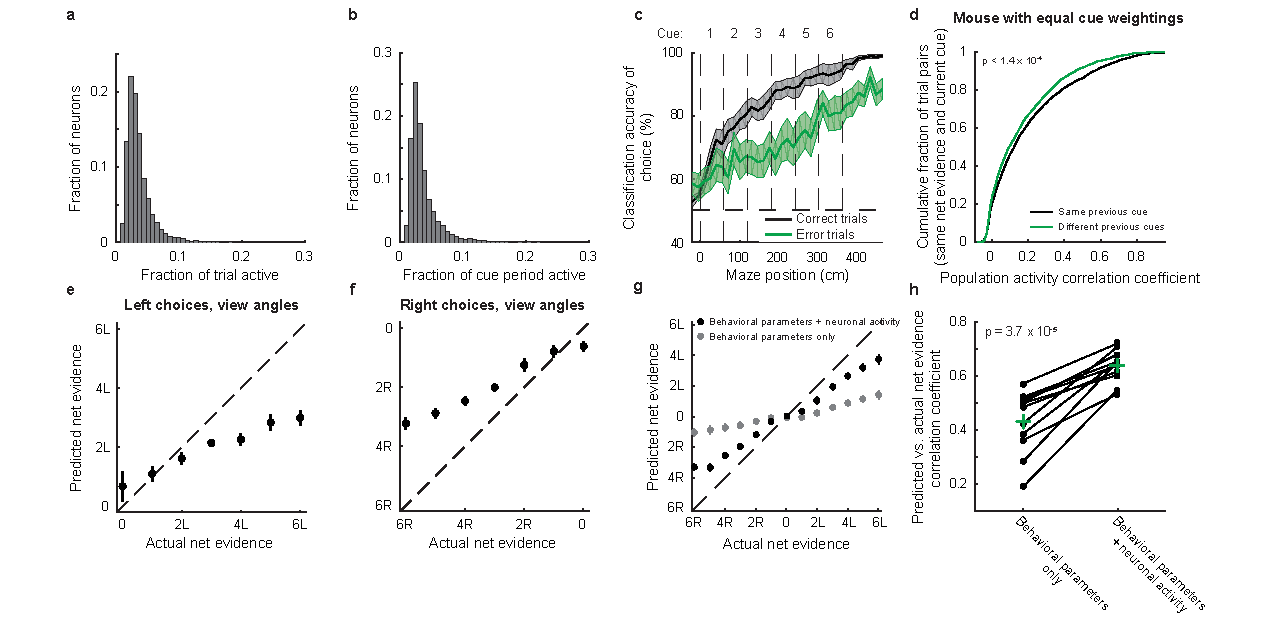
\includegraphics[width=1\textwidth,center]{figures/fig_3_5.pdf}
\caption[Analyses of single neuron- and population-level representations of task-relevant features.]
{\textbf{Analyses of single neuron- and population-level representations of task-relevant features. a-b,} Histogram of the fraction of the entire trial (\textbf{a}) and cue period (cues 1-6) (\textbf{b}) neurons were active (n = 3840 neurons from 5 mice). 
%
\textbf{c,} SVM classification accuracy (mean $\pm$ s.e.m., n = 11 datasets) for choice based on population activity on correct and error trials. Independent classifiers were trained and tested at each maze position. 
%
\textbf{d,} Same as Figure \ref{fig:3_15}a except for a mouse with equal cue weightings. Cumulative distribution of the pairwise trial-trial population activity correlation coefficients for epochs with the same (black) or different (green) previous cues, keeping net evidence and epoch constant (e.g., \textit{LRLXXX} vs. \textit{RLLXXX} trials at cue 3) (p < 1.4 x 10-4, two-sample KS test, n = 2 datasets; mouse colored as red in Figures \ref{fig:2_2}, \ref{fig:2_4}b, d). This analysis tested if neuronal activity at a given epoch contained information about the previous epoch's cue, independent of maze epoch and net evidence. 
%
\textbf{e-f,} SVR classifiers for net evidence performed on trials with nearly identical ($\pm$ 2.5\textdegree) view angles on left choice (\textbf{e}) and right choice (\textbf{f}) trials. Across mice the predicted vs. actual net evidence correlation coefficient was significantly higher for the model with behavioral parameters and neuronal activity than for the model with behavioral parameters only (p < 0.001 relative to shuffled net evidence labels). Net evidence therefore appeared decodable beyond information provided by view angle.
%
\textbf{g,} Actual net evidence vs. net evidence predicted by an SVR classifier trained on behavioral parameters only (gray) or both behavioral parameters and neuronal population activity (black) (Methods \ref{methods:multi_class_classifications}). Error bars represent mean $\pm$ s.e.m. across datasets (n = 11). 
%
\textbf{h,} Data from (\textbf{g}) shown for individual datasets. Green crosses represent means across datasets (n = 11). 
\label{fig:3_5}}
\end{figure}

\bigskip
The choice and net evidence information might have come solely from a small fraction of neurons with high selectivity; these are the neurons that we and others have emphasized previously. Alternatively, information could have been distributed across a large group of neurons extending beyond the classically selective neurons. To distinguish these possibilities, we applied the population activity classifiers for choice and net evidence to increasingly larger subsets of neurons, beginning with neurons with the lowest individual classification accuracy. The accuracy of both classifiers increased with the incorporation of neurons that individually represented choice and net evidence poorly (Figure \ref{fig:3_3}g-h). Using the 40\% least selective neurons, we were able to predict the mouse’s choice with 75\% accuracy, even though none of these neurons had a statistically significant choice selectivity index (Figure \ref{fig:3_3}g). The improvement with the addition of more neurons could have resulted from the additive effect of weak information in each neuron or the revelation of correlated activity patterns with the addition of larger numbers of neurons or both; we plan to investigate these possibilities in future work. Together, these results suggest a population representation in which information is distributed across heterogeneous and variable neurons, as has been suggested previously in studies of coding in individual neurons \citep{Meister:2013ca, Park:2014co, Jun:2010kj, Raposo:2014df, Mante:2013ie, Rigotti:2013bo, Maimon:2009hg, Churchland:2010he}. For all subsequent analyses, we therefore considered all the neurons we imaged, in contrast to many previous studies that have selected, either at the measurement or analysis stage, only those neurons that were individually selective for a specific task feature, such as choice.

\subsection{Clustering neuronal activity patterns across trials} \label{sec:chap3_clustering}

Given that neuronal activity was in large part heterogeneous across neurons and variable between trials and that task-relevant information was distributed across neurons, we reasoned that further analyses of individual neuron activities might not achieve our goal of understanding features of the population activity on single trials. We therefore focused our subsequent analyses exclusively on the population level by developing methods to measure how the population activity pattern changed from moment to moment. We defined the population activity pattern at a given time period as the vector of each neuron’s estimated spike count in that period. We conceptualized the population activity as a trajectory involving transitions from one activity pattern to another. To facilitate the analysis and visualization of transitions between patterns over time, we reduced the dimensionality of the population activity using a clustering algorithm. Activity patterns were clustered based on similarity in the \textit{n}-dimensional activity space defined by the \textit{n} simultaneously imaged neurons (Methods \ref{methods:clustering_general}). We considered each cluster to represent an activity pattern in the PPC population. The number of clusters was determined using the affinity propagation clustering algorithm \citep{Frey:2007tj}. Our results were consistent across a wide range of cluster numbers and affinity propagation settings (Figure \ref{fig:3_7}k; Methods \ref{methods:clustering_affinity}). Clustering was performed independently for ten epochs, each of which corresponded to a different time period of the trial. For each epoch, the estimated spike count on each of\textit{ m }trials for each of \textit{n} simultaneously imaged neurons was calculated, resulting in \textit{m} points in an \textit{n}-dimensional space. We clustered these m points such that each cluster corresponded to a different set of trials with similar population activity patterns at a given epoch (11 $\pm$ 8.4 trials/cluster on average; Figure \ref{fig:3_7}e). Each trial was part of a single cluster at each epoch. For visualization, each cluster was represented as a circular node with area proportional to the number of trials in the cluster (Figure \ref{fig:3_6}e). Transitions between clusters in consecutive epochs were marked as lines with thickness proportional to the transition probability (Methods \ref{methods:clustering_trans_prob}). Single trials could therefore be described as an activity trajectory defined by the sequence of clusters visited from epoch to epoch. These cluster-space trajectories are conceptually identical to trajectories that have previously been described using principal component analysis and other methods; the only difference is in the dimensionality reduction algorithm used \citep{Harvey:2012du, Churchland:2012bq, Mante:2013ie, Mazor:2005jp, Briggman:2005jd, Raposo:2014df}.

% THIS IS A FULL PAGE FIGURE
\begin{FPfigure}
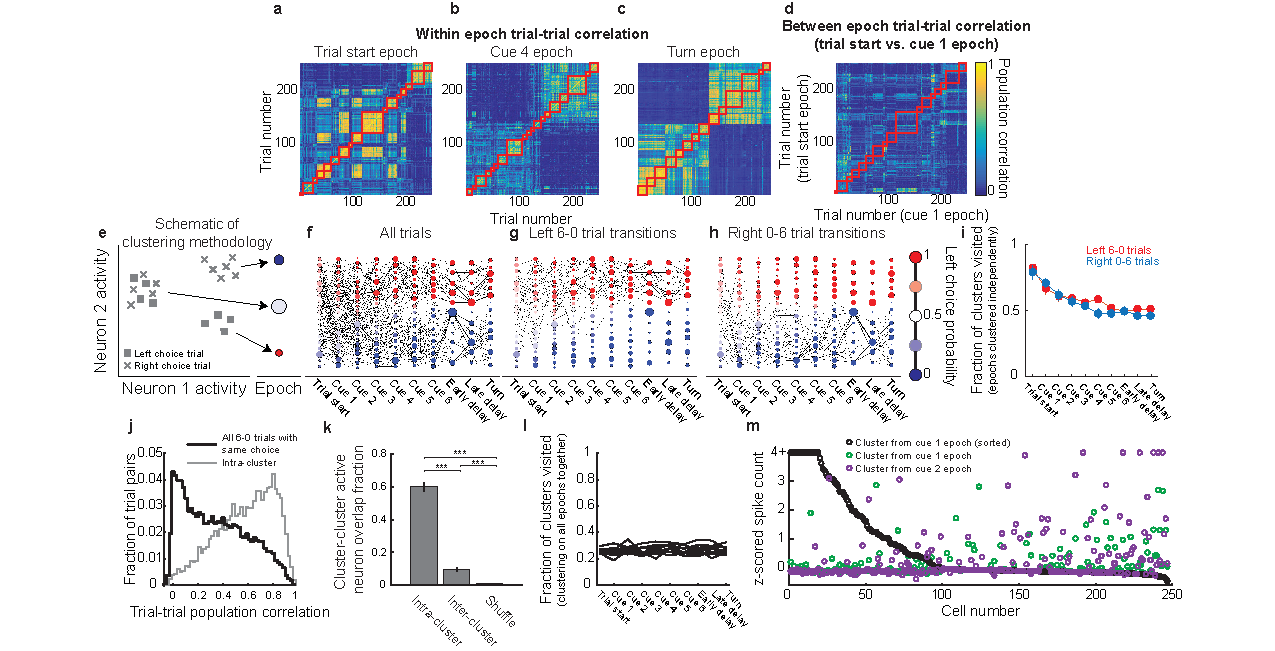
\includegraphics[width=1.2\textwidth,center]{figures/fig_3_6.pdf}
\caption[Clustering neuronal activity across trials to reveals trial-to-trial variability.]
{\textbf{Clustering neuronal activity across trials to reveals trial-to-trial variability. a-c,} Example trial-trial population activity correlation matrices at the trial start epoch (\textbf{a}),  cue 4 epoch (\textbf{b}), and the turn epoch (\textbf{c}) sorted by cluster identity. Red squares indicated cluster membership such that pairs of trials within the same red square were in the same cluster. 
%
\textbf{d,} Example trial-trial population activity correlation matrix for two consecutive epochs (trial start epoch compared to cue 1 epoch). Trials were sorted according to the cluster identity during the trial start epoch. Because trials were sorted identically in both epochs, trial pairs along the diagonal would be expected to have high correlations if trial activity was similar in consecutive epochs. In contrast, the low correlations along the diagonal suggest that trials had highly different population activity in consecutive epochs.
%
\textbf{e,} Schematic demonstrating clustering procedure (Methods \ref{methods:clustering_general}). At each of ten spatially-defined maze epochs, clustering was used to group together individual trials with similar population activity patterns. Clusters at each maze epoch were represented as a column of nodes with area proportional to the number of trials in each cluster. Nodes were colored based on the fraction of trials within each cluster resulting in a left choice. Nodes were sorted vertically from largest to smallest left choice probability. Transition matrices were constructed by calculating the empirical transition probability between adjacent clusters. 
%
\textbf{f,} An example transition matrix constructed from all trials in a single dataset. Edge widths between nodes represent the forward transition probability. Nodes were colored and sorted as described in (\textbf{e}). 
%
\textbf{g-h,} Transition probabilities for left 6-0 (\textbf{g}) and right 0-6 (\textbf{h}) trials using the same clusters derived from all trials as in \textbf{f}. Despite identical cues and choices, the paths through the transition matrix of each group were highly variable. 
%
\textbf{i,} Fraction of clusters visited by left 6-0 (red) and right 0-6 (blue) trials at each epoch decreased to only 0.5, suggesting that much variability remained among these trials, even at the turn. 
%
\textbf{j,} Distribution of pairwise trial-trial population activity pattern correlations for pairs of trials with identical cues and choices at the turn epoch for all 6-0 trials (black) and only trial pairs in the same cluster (gray). 
%
\textbf{k,} Mean overlap fraction of active neurons within the same cluster (intra-cluster) and across clusters (inter-cluster). The overlap fraction was defined as: (number of neurons active in both clusters / number of neurons active in either cluster). Small inter-cluster overlap suggested that a largely distinct group of neurons was active in each cluster. Overlap fractions were calculated separately for correct left 6-0 and right 0-6 trials. Shuffled overlap index was calculated by shuffling the assignment of trials to clusters. Cells with activity exceeding a z-score threshold of 1.5 were considered `active'. ***P < 0.001, two-sample Student's t-test. Error bars represent mean $\pm$ s.e.m. across datasets. 
%
\textbf{l,} Fraction of clusters visited at a given epoch when clustering was performed on all epochs together (Methods \ref{methods:clustering_together}). All trial types were included. Individual lines represent datasets (n = 11). The fraction of clusters visited was similar at all epochs, even at the turn epoch. 
%
\textbf{m,} z-scored activity of cells in two clusters during correct left 6-0 trials at the cue 1 epoch (black and green) and one cluster at the cue 2 epoch (purple). Cells were sorted according to their activity in the black cluster, such that the cell numbers were the same for each displayed cluster. 
\label{fig:3_6}}
\end{FPfigure}
%\afterpage{\clearpage}
\clearpage

\bigskip
Before exploring population dynamics in the cluster space, we first sought to gain an intuition of how neuronal activity patterns related to the clusters. We visualized the relationship between neuronal activity and clusters by calculating for each pair of trials the correlation between their population activity patterns at a given epoch. We sorted the matrix of trial-trial correlation coefficients by the trials that were clustered together (Figure \ref{fig:3_6}a-c). This visualization revealed that clustering identified structure in the trial-trial activity pattern correlations and showed that clusters varied over a wide distribution in how similar they were to one another. As expected by the transient activity we observed in individual neurons (Figures \ref{fig:3_3}a, \ref{fig:3_4}, \ref{fig:3_5}a-b), the activity patterns in clusters at one epoch were largely different from the activity patterns observed in clusters at the subsequent epoch (Figures \ref{fig:3_6}d, \ref{fig:3_9}f). Consistently, when we clustered activity patterns from all epochs together, rather than for single epochs individually, such that the clusters were the same from epoch to epoch, we found that the likelihood of a trial staying in the same cluster across consecutive epochs was rare (0.9 $\pm$ 0.01\% of transitions; Figure \ref{fig:3_7}f; Methods \ref{methods:clustering_together}). The activity patterns in each cluster were made up of complex combinations of activity levels in the population of individual neurons. Some individual neurons thus had elevated activity in multiple clusters (Figures \ref{fig:3_6}m, \ref{fig:3_7}i-j, \ref{fig:3_8}). A cluster should therefore be considered as a pattern of activity across neurons in the population, such that the patterns between clusters are discriminable from one another.  Future work will aim to identify the structure of these activity patterns within clusters, but, importantly, for the focus of this work, clusters were primarily considered an abstracted grouping of similar activity patterns, and the precise activity patterns that defined each cluster were not important for the subsequent analyses and results.

\bigskip
Activity patterns reflecting important task-relevant features, including choice and net evidence, were apparent in the cluster space, even though clustering was performed on neuronal activity alone without any information about behavioral parameters (Figure \ref{fig:3_7}a-d). For choice, for example, different paths through clusters emerged for left- and right-choice trials, which is a visualization of the choice-specific activity trajectories we observed previously \citep{Harvey:2012du} (Figure \ref{fig:3_6}f-h). 

\bigskip
We used the cluster space to visualize the population activity trajectories on single trials. This visualization revealed a high amount of trial-trial variability. Trials with the same choice, even during the turn epoch, occupied a diverse set of clusters and traversed different paths through cluster space, suggesting they had distinguishable activity patterns and trajectories. This variability could have been caused by differences in the sequences of cues presented on different trials. We therefore focused on trials with identical evidence cues and choices (e.g., correct 6-0 left trials), which were randomly interleaved with other evidence accumulation trials during imaging (5-1, 4-2, and 3-3 trials).  Trials of the same type might be expected to have highly correlated activity patterns and thus converge to similar paths through a small set of clusters. In contrast, the population of trials with identical evidence cues and choices occupied more than half of all possible clusters at each epoch, even at the turn after a choice was made (Figure \ref{fig:3_6}g-i).


%\begin{figure}
\begin{FPfigure}
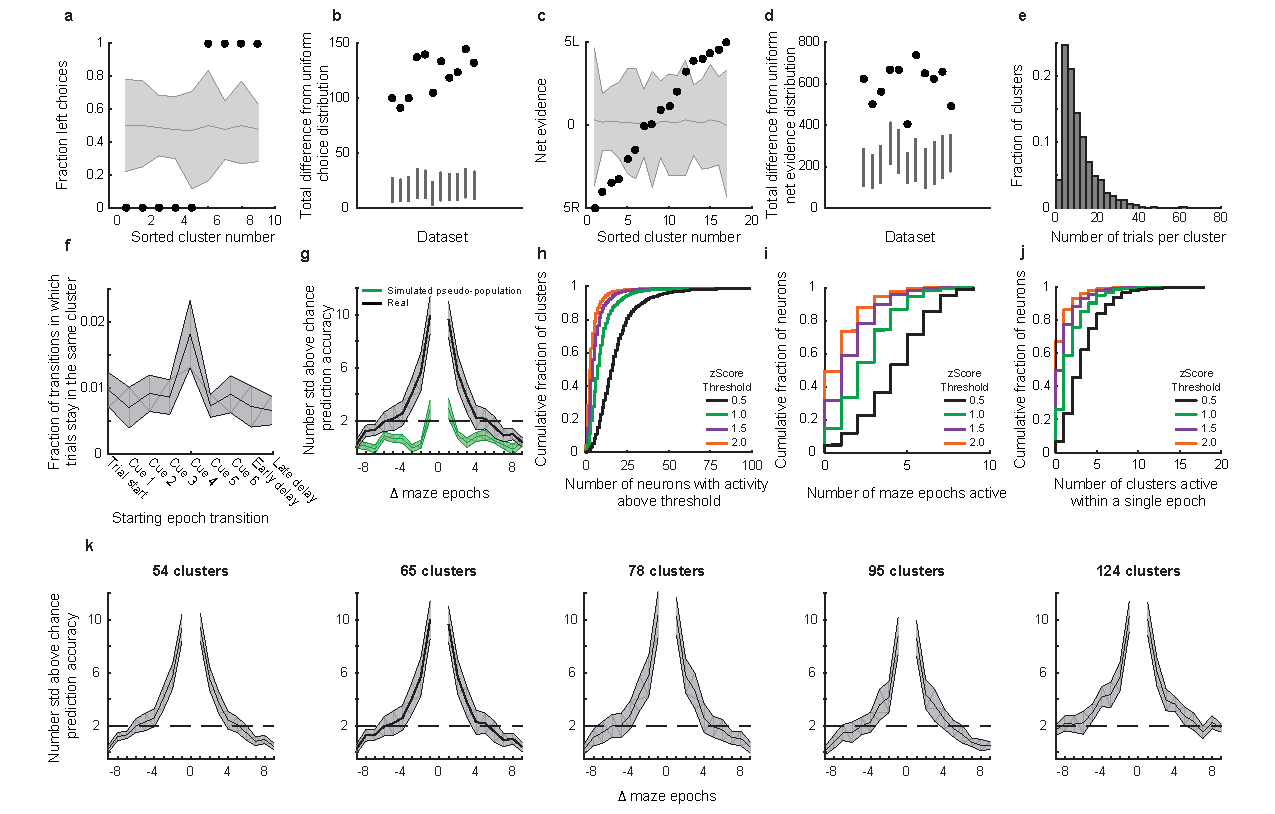
\includegraphics[width=1.1\textwidth,center]{figures/fig_3_7.pdf}
\caption[Characterization of behavioral and neuronal patterns across clusters.]
{\textbf{Characterization of behavioral and neuronal patterns across clusters. a,} Fraction of trials in each cluster in the turn epoch that were left choice trials for an example dataset. Clustering revealed neuronal activity patterns related to behavioral choices. Gray area indicates the median and 99\% confidence intervals of the shuffled distribution of trial assignments to clusters.  
%
\textbf{b,} Comparison of the total difference from a uniform distribution for the real data (circles) to the 99\% confidence intervals of the corresponding shuffle for each dataset (lines). The total difference was calculated as the summed absolute difference from the shuffle median across clusters.
%
\textbf{c-d,} Same as in \textbf{a-b,} but for net evidence during the fifth cue. 
%
\textbf{e,} Distribution of trials per cluster across all epochs and datasets (n = 2457 clusters). 
%
\textbf{f,} Cluster self-transition probabilities for clustering performed using all epochs together. Transition probabilities were considered from one epoch to the next epoch. Low self-transition probabilities suggested that activity patterns changed over the time of consecutive epochs. Error bars represent mean $\pm$ s.e.m across datasets. 
%
\textbf{g,} Based on the cluster identity for a trial at a given epoch, the accuracy of predicting the clusters that trial occupied in the past and future. Real data are shown in black and a simulated pseudo-population is shown in green. To create the pseudo-population, trial identities were shuffled independently for each neuron to break neuron-neuron correlation structure but to preserve each neuron's activity within the trial (Methods \ref{methods:clustering_pseudopop}). Error bars represent mean $\pm$ s.e.m. across datasets. 
%
\textbf{h,} Cumulative distribution of the number of neurons active in each cluster for different z-score activity thresholds. 
%
\textbf{i,} Cumulative distribution of the number of maze epochs in which a neuron was active in at least one cluster for different z-score activity thresholds. 
%
\textbf{j,} Cumulative distribution of the number of clusters in which a neuron was active within a single epoch for different z-score activity thresholds. 
%
\textbf{k,} For a given trial based on the current cluster identity, the accuracy of predicting the clusters occupied by that trial in the past and future epochs did not depend greatly on the clustering preference parameters (percentile of the distance matrix used for clustering; 1\textsuperscript{st}, 10\textsuperscript{th}, 30\textsuperscript{th}, 50\textsuperscript{th}, 70\textsuperscript{th} from left to right) and, hence, numbers of clusters. Cluster numbers are the mean number of clusters for each preference parameter across datasets. Error bars represent mean $\pm$ s.e.m. across datasets. 
\label{fig:3_7}}
%\end{figure}
\end{FPfigure}
%\afterpage{\clearpage}
\clearpage

This initial visualization of single trials in cluster space revealed that different trajectories emerged for different trial types (e.g., left vs. right choice) and that within each trial type extensive variability was present, consistent with previous studies of variability in the activity of cortical neurons \citep{Britten:1992wx, Renart:2014drba, Marcos:2013byba, Churchland:2010he, Churchland:2011hd, Maimon:2009hg}.

\bigskip
Although the variability in the clusters occupied revealed that trials had distinguishable activity patterns at a given epoch, we wanted to gain more insight into the neuronal basis of this variability. For example, trial-trial variability could have resulted from modulations of the tonic firing of all neurons or from major changes in which sets of neurons were active in each trial. As a first examination of the variability, for each pair of clusters in a given epoch, we calculated the fraction of neurons that were active in both clusters (active neurons were defined by a threshold in z-scored estimated spike counts: threshold = 1.5). Surprisingly, only 10\% of neurons on average were active in both clusters, even when limiting our analysis to trials with identical choices and evidence cues. Many trials of the same type therefore had largely non-overlapping populations of active neurons (Figures \ref{fig:3_6}k, \ref{fig:3_8}). Consistently, the correlation coefficient between the population activity patterns for pairs of trials of the same type at the same epoch (e.g., 6-0 left trials at the turn period) had a wide distribution. Some trial pairs had highly correlated activity, and others had correlation coefficients near zero (Figure \ref{fig:3_6}a-c, j). In addition, we quantified the variability as a function of time in the trial using the cluster space defined by clustering activity patterns from all epochs together, rather than clustering independently within each epoch (Methods \ref{methods:clustering_together}). The variability was estimated at a given epoch as the fraction of clusters explored by a population of trials. Surprisingly, when considering all trial types together, the fraction of clusters visited did not decrease over the course of the trial (Figure \ref{fig:3_6}l). The activity therefore maintained a high number of distinguishable activity patterns throughout the trial and did not collapse to a low-variability representation even at the turn epoch after a choice had been made. Together, these results suggest that individual trials with the same cues and choices varied greatly to the extent of having largely non-overlapping sets of active neurons.


\begin{figure}
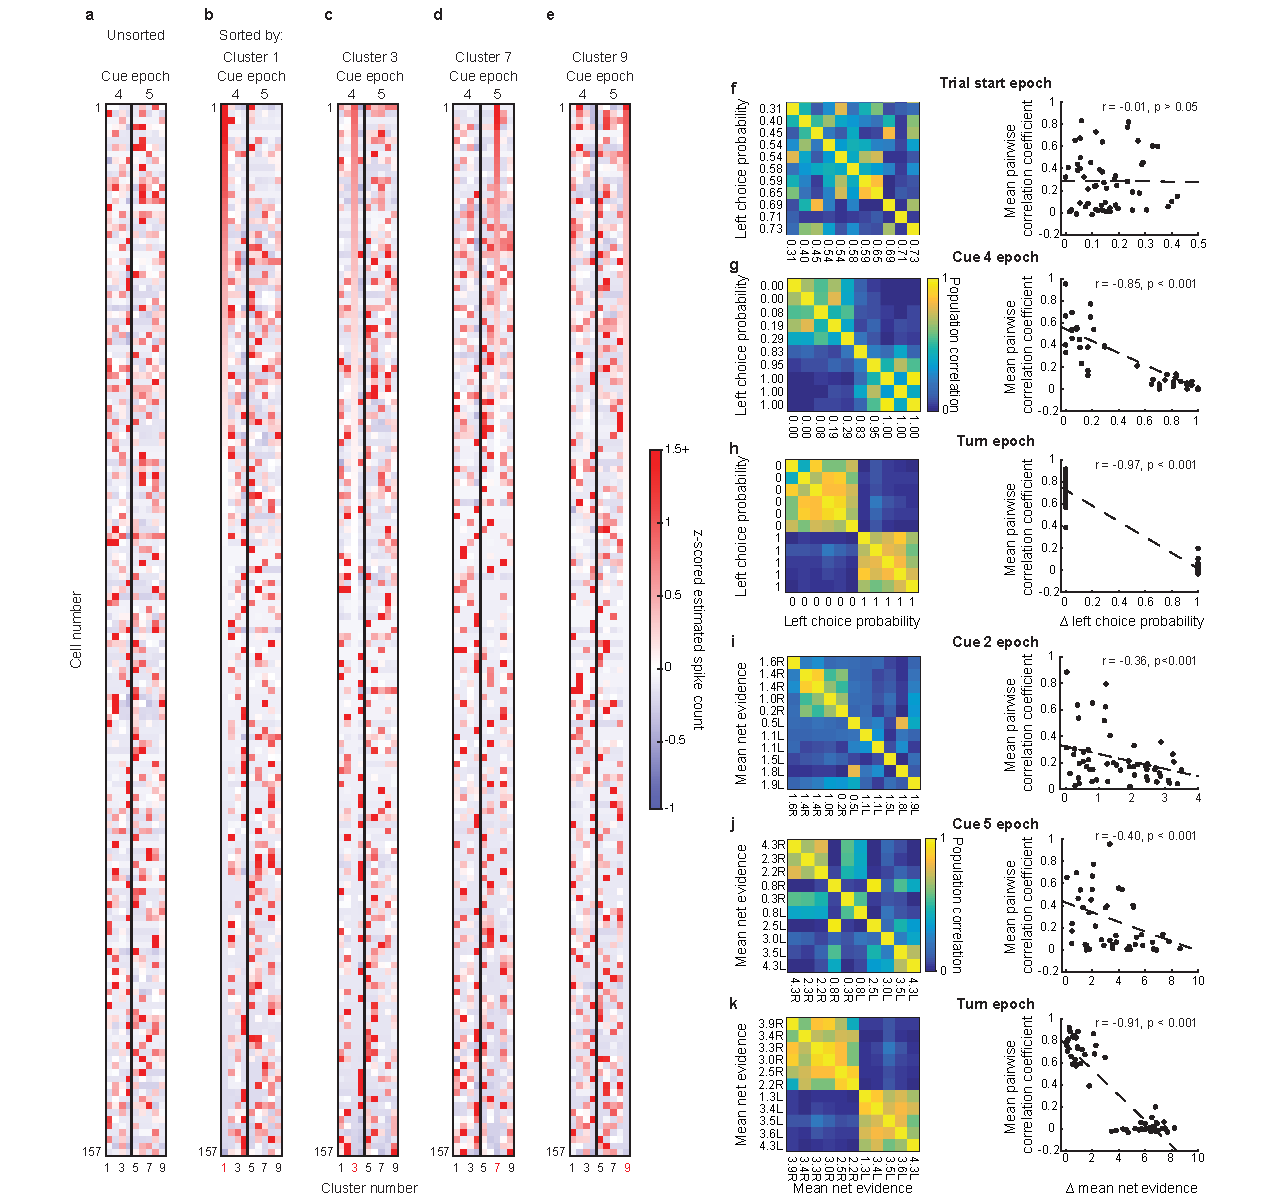
\includegraphics[width=1\textwidth,center]{figures/fig_3_8.pdf}
\caption[Visualizations of neuronal activity across clusters.]
{\textbf{Visualizations of neuronal activity across clusters. a-e,} Mean z-scored spike count for individual neurons across clusters comprised only of correct left 6-0 trials at two adjacent epochs (Cues 4 and 5) from a single dataset. These plots demonstrate that the activity across clusters and epochs featured largely different patterns of active neurons. Neurons were either unsorted (\textbf{a}) or sorted according to their activity in clusters 1, 3, 7, or 9 (\textbf{b-e}). Neurons whose mean z-scored activity was less than 0.001 in all of the displayed clusters were excluded for display purposes (these neurons were active during a different trial epoch). Clusters were generated from correct left 6-0 trials.
%
\textbf{f-h,} Left panels: Matrix of population activity correlations between each pair of cluster centers sorted according to the cluster's left choice probability at three different maze epochs. For each cluster, the population activity was calculated as the mean activity vector across trials for each cluster. Right panels: Population activity correlation between each pair of clusters as a function of their difference in left choice probability.  
%
\textbf{i-k,} Same as in \textbf{f-h,} but for net evidence. 
\label{fig:3_8}}
\end{figure}

\subsection{Temporally structured trial-trial variability} \label{sec:chap3_temp_struc}

Given that a stereotyped sequence of activity patterns was not present for trials with identical cues and choices, we sought to understand the cause of the trial-trial variations. We therefore focused only on trials of a single type in order to remove the variability due to differences in trial events (e.g., different evidence cues and choices). Using only trials of a single type (e.g., left 6-0 or right 0-6 trials), we generated a new cluster space to examine the within trial type variability (Figure \ref{fig:3_9}a). The variability in activity trajectories in this case could be due predominantly to biological or measurement noise. If so, the transitions from one activity pattern to the next are expected to be unpredictable, such that each single trial wanders through a random sequence of activity patterns. Alternatively, the variability between trials of the same type could carry information. In this case, each trial is expected to traverse an orderly set of activity patterns, such that the transition from one activity pattern to the next is predictable. To examine these possibilities, we tested if we could predict the future activity patterns of a trial based on the trial’s current activity pattern. As a first test, we visualized the paths of trials starting from a single cluster and found that only a subset of subsequent clusters was visited by those trials, even at many epochs later in the trial (Figure \ref{fig:3_9}b). This example suggests that by knowing the trial’s starting point, we could predict, to some extent, the clusters visited by that trial in the future, which is consistent with structure in the activity pattern transitions across time. To visualize if this structure could occur by chance, we simulated a ‘noise’ case by shuffling the assignment of trials to clusters at each epoch (maintaining the distribution of trials across clusters), thus creating transitions between clusters that mimic noise-driven transitions. In the shuffled (‘noise’) case, the trials starting in a single cluster visited all subsequent clusters, in contrast to what we observed in the real data (Figure \ref{fig:3_9}c).
 

\begin{figure}
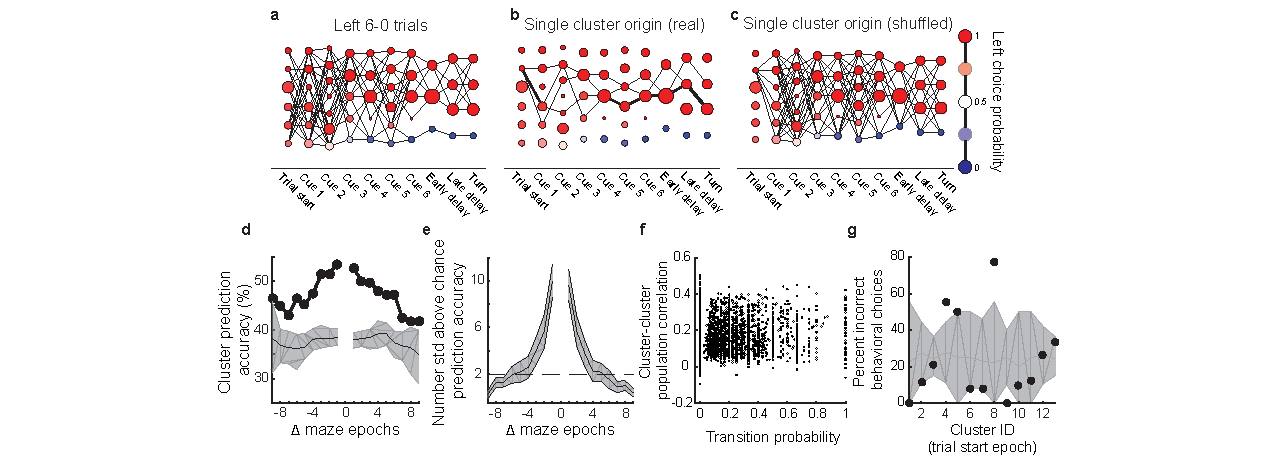
\includegraphics[width=1.5\textwidth,center]{figures/fig_3_9.pdf}
\caption[Long timescale temporal structure in PPC activity.]
{\textbf{Long timescale temporal structure in PPC activity. a,} Example transition matrix constructed only from left 6-0 (both correct and error) trials in a single dataset. The nodes at the trial start had high left choice probabilities, even before evidence cues were presented, because the only trials included in this analysis were left 6-0 trials, which almost always resulted in a left choice.
%
\textbf{b-c,} Transition probabilities of all trials starting from a single cluster for real (\textbf{b}) and shuffled (\textbf{c}) data. In shuffled data, the assignment of trials to clusters was randomized, maintaining the distribution of trials across clusters.
%
\textbf{d,} Based on the cluster identity for a trial at a given epoch, the accuracy of correctly predicting that trial's past and future cluster occupancies (Methods \ref{methods:clustering_past_future_class}). Predictability across many epochs suggests long timescale temporal structure in single trial activity trajectories. Accuracies were pooled across left 6-0 and right 0-6 trials that were clustered and considered separately. Error bars represent the median and 99\% confidence intervals from data in which the assignment of trials to clusters was shuffled. 
%
\textbf{e,} Same as in \textbf{d}, but averaged across all datasets (n = 11). To combine across datasets with different chance classifier performance, accuracies were converted into the number of standard deviations above the shuffled distribution. Error bars represent mean $\pm$ s.e.m. across datasets. 
%
\textbf{f,} Relationship between the population activity correlation of clusters in adjacent epochs and the transition probability between them. Transitions were not more likely between clusters with more similar population activity patterns (r = 0.02, p > 0.05).
%
\textbf{g,} Distribution of behavioral error probabilities (i.e. error trials in a cluster divided by total trials in a cluster) across clusters at the trial start for a single dataset. Error bars represent 99\% confidence intervals of data in which the assignment of trials to clusters was shuffled. Because many of the clusters contain substantially more or fewer error trials than the shuffled distribution, this distribution is significantly different than chance (p < 0.01). For example, trials beginning in cluster 8 result in an error trial close to 80\% of the time. Similar results were observed in other datasets.
\label{fig:3_9}}
\end{figure} 


\bigskip
This example suggested that the transitions between activity patterns could be non-random and that temporal structure might exist in the variable paths traversed by single trials of the same type. We quantified this structure by developing a classifier in cluster space that asked if, based on the identity of the cluster occupied by a given trial at the current epoch, we could predict the identities of the clusters occupied by that same trial in past and future epochs. This analysis therefore tests if the current activity pattern contained information about past and future activity patterns within a single trial. For trials with identical choices and evidence cues, the classifier predicted significantly above chance which cluster a trial occupied $\sim$5-6 epochs ($\sim$4-5 seconds) into the past and future, and in some cases across the entire trial (Figure \ref{fig:3_9}d-e).  Similar predictability was observed in the \textit{n}-dimensional activity space (Figure \ref{fig:3_10}a-b; Methods \ref{methods:offset}). In addition, the vector describing the change in population activity in response to a new cue was also dependent on the current activity pattern, which suggests that dynamics in the population activity affected how inputs influenced ongoing network activity (Figure \ref{fig:3_10}c-d; Methods \ref{methods:vector}). We performed extensive tests to ensure that the temporal structure was not imposed by the clustering process (Methods \ref{methods:clustering_pseudopop}). 


\begin{figure}
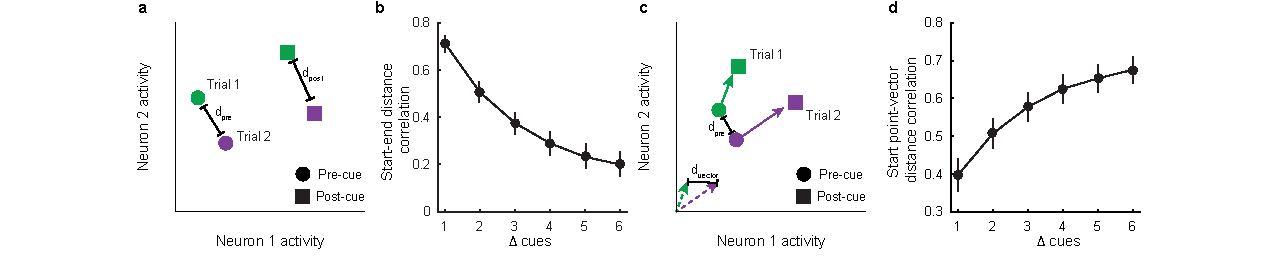
\includegraphics[width=1.1\textwidth,center]{figures/fig_3_10.pdf}
\caption[Influence of the current population activity pattern on future population activity patterns and the change in population activity in n-dimensional activity space.]
{\textbf{Influence of the current population activity pattern on future population activity patterns and the change in population activity in n-dimensional activity space. a,} Schematic illustrating the distances between two trials before (d\textsubscript{pre}) and after (d\textsubscript{post}) a cue was presented. \textbf{b,} Pairwise correlation coefficients between the starting and ending distances across trials with identical cues presented and for different numbers of cues ($\Delta$cues) between the start and end points. At all $\Delta$cues, correlation coefficients were significantly different from a shuffled distribution (Methods \ref{methods:offset}; p < 0.001), showing that the distance between trials before an identical sequence of cues is presented is predictive of their distance after the cues are presented. Error bars represent mean $\pm$ s.e.m. across datasets. \textbf{c,} Schematic illustrating the starting (d\textsubscript{pre}) distance between two trials and the distance between each trial’s vector resulting from cue presentation (d\textsubscript{vector}). \textbf{d,} Pairwise correlation coefficients between the starting distance and vector distance across trials with identical cues presented.  Correlation increased with $\Delta$cues. At all $\Delta$cues, correlation coefficients were significantly different from a shuffled distribution (Methods \ref{methods:vector}; p < 0.001), suggesting that the vector defining the change in population activity in response to a cue depends on both the cue and the starting population activity pattern. Error bars represent mean $\pm$ s.e.m. across datasets.
\label{fig:3_10}}
\end{figure} 


\bigskip
It is also possible that trial-trial differences in behavioral parameters could have generated the structured trial-trial variability in neuronal activity and the presence of history signals across long timescales. We ruled out these possibilities using a series of tests to see if neuronal activity explained additional variability beyond what could be explained by the behavioral variability, by building both neuronal activity and behavioral features into a single logistic regression model (Methods \ref{methods:clustering_behav_past_future}. We found that the current behavioral parameters (view angle, maze position, treadmill rotational velocity, which together define the visual scene and running patterns) alone explained above chance, but poorly, past and future activity pattern clusters for only 1 epoch into the past or future (Figure \ref{fig:3_11}). In contrast, models using the current behavioral parameters and the current activity pattern cluster (or the current activity pattern alone) predicted the past and future epochs significantly better, including across a longer timescale of $\sim$5-6 epochs (determined by adjusted R\textsuperscript{2} to compare models with different numbers of parameters; Figure \ref{fig:3_11}). Together, these results indicate that the current activity pattern contained information about past activity patterns and influenced the transition probabilities to future activity patterns, even when removing the effects of different trial events like evidence cues and choice.


%FIGURE 3_11
\begin{figure}
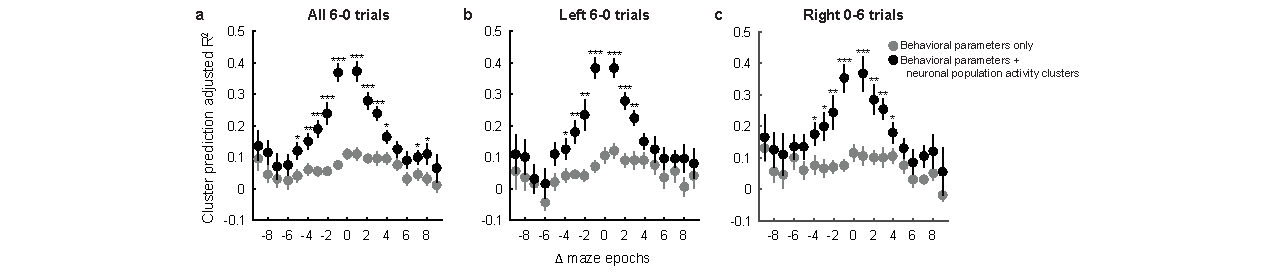
\includegraphics[width=1.4\textwidth,center]{figures/fig_3_11.pdf}
\caption[Contribution of behavioral variability to temporally structured trial-trial variability.]
{\textbf{Contribution of behavioral variability to temporally structured trial-trial variability.}  Our ability to predict the past and future population activity pattern based on the current population activity pattern could not be explained by behavioral variability. We performed a multivariate logistic regression to predict a trial's cluster identity at a given epoch based on only the behavioral parameters at another epoch (gray) or both the behavioral parameters and the cluster identity at another epoch (black). To allow for a binary classifier, we only included those trials whose cluster identity contained either the most or second most trials during the prediction epoch (Methods \ref{methods:clustering_behav_past_future}). Consistently, the model based on both behavioral parameters and the neuronal population cluster identity outperformed the model based on only behavioral parameters. This analysis was performed on left 6-0 trials (\textbf{b}) and right 0-6 trials (\textbf{c}) separately, and the results were pooled together to generate the plot for all 6-0 trials (\textbf{a}). The behavioral parameters used were x/y position, x/y treadmill velocity, and view angle as described in Section \ref{sec:vr}.  Separate models were fit for each combination of previous and future cluster identities and combined based on the number of maze epochs between them ($\Delta$ maze epochs). Adjusted R\textsuperscript{2} values were used to compare the predictive power of models with different numbers of explanatory variables. *P < 0.05, **P < 0.01, ***P < 0.001, two-sample Student's t-test.
\label{fig:3_11}}
\end{figure} 

\bigskip
The long timescale temporal structure we observed could be caused by multiple factors. First, this structure could arise from persistent activity patterns, in which single neurons have long-lasting activity across epochs. Alternatively, there may exist predictable progressions between time-varying activity patterns, such that the PPC has long timescale dynamics via structured transitions from one short-lived population activity pattern to another. Multiple features of the data provided strong support for the second alternative. We found that neurons were transiently active with time-varying activity (Figures \ref{fig:3_3}a, \ref{fig:3_4}, \ref{fig:3_5}a-b). Also, clusters from different epochs had mostly distinct activity patterns (Figure \ref{fig:3_6}d, \ref{fig:3_9}f). Furthermore, transitions were just as likely between clusters with similar activity patterns as they were between clusters with dissimilar activity patterns (Figure \ref{fig:3_9}f). As an additional test of whether the long timescale structure could have emerged from long-lasting activity in individual neurons, we shuffled the trial identities separately for each neuron among trials of the same type. This shuffle broke neuron-neuron correlation structure but preserved activity patterns in individual neurons (simulating a pseudo-population). The removal of neuron-neuron correlations eliminated our ability to predict the past and future clusters visited by a single trial based on the current cluster occupied by that trial (Figure \ref{fig:3_7}g). Together these results indicate that the temporal structure in single trials did not arise from long-lasting activity in individual cells; rather, structured moment-to-moment transitions occurred between transient patterns of neuronal activity with largely different sets of active neurons.

\bigskip
Given that long timescale structure existed in PPC activity, we considered the possibility that activity patterns may be predictive of behavioral outcomes long in advance. To test this possibility, we asked if the population activity pattern, even before the first cue was presented, was related to if the mouse made a correct or incorrect choice (Methods \ref{methods:clustering_behav_error}). We found that even before the mouse had seen any evidence cues, a small set of clusters contained significantly more error trials than would be expected by chance, suggesting that the activity patterns associated with those clusters were predictive of incorrect choices later in the trial (p < 0.001; Figure \ref{fig:3_9}g). Also, using an SVM classifier, we could predict the mouse’s choice on error trials, but not on correct trials, weakly above chance before any cues were presented (p < 0.01 at the first bin a trial; Figure \ref{fig:3_5}c).

\subsection{A memory of past events is maintained in PPC population activity over seconds and across trials} \label{sec:chap3_past_events}

Thus far, our results indicate that long timescale structure exists in the PPC over seconds, not as sustained activity in individual neurons but rather as orderly transitions from one activity pattern to another, often with large variations in which neurons were active. We have shown, based on our ability to predict past and future activity patterns from the current activity, that the activity pattern at a given moment contained information about past activity patterns and also influenced the transition probabilities to future activity patterns over seconds. These results make important predictions about the timescale over which information about transient events is maintained in the PPC. An event during a trial is expected to result in a new population activity pattern. This new activity pattern would depend on both the features of the event and the activity pattern transition probabilities immediately prior to the event. Because of the long temporal structure that we identified in PPC dynamics, the activity pattern following the event is then expected to influence the transition probabilities to future activity patterns. Because the event helped to generate this new activity pattern, and because this activity pattern influences the transition probabilities to future activity patterns, the event also has an effect on the transition probabilities to future activity patterns. Therefore, by helping to create the activity pattern in the population, a transient event is expected to have a long-lasting effect by constraining the possible future activity patterns. We therefore hypothesized that transient events have signatures of their occurrence long after they ended. In this case, the variability we observed between trials of the same type could have emerged as a consequence of differences in recent past events.

%FIGURE 3_12
\begin{figure}
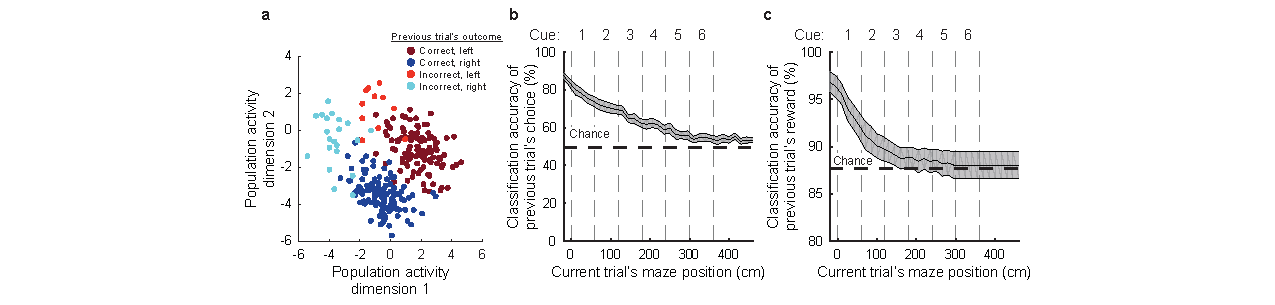
\includegraphics[width=1.6\textwidth,center]{figures/fig_3_12.pdf}
\caption[Neuronal population activity in the current trial reflects the previous trial's choice and outcome.]
{\textbf{Neuronal population activity in the current trial reflects the previous trial's choice and outcome. a,} Population activity patterns on different trials at the trial start epoch colored by the choice and outcome (reward or no reward) of the previous trial. Dimensionality was reduced using factor analysis for visualization purposes. Each circle is one trial. 
%
\textbf{b-c,} Both the previous trial's choice (\textbf{b}) and if the previous trial was rewarded (\textbf{c}) could be classified based on the population activity. Independent SVM classifiers were trained and tested at each maze position. Error bars represent mean $\pm$ s.e.m. across datasets (n = 11).
\label{fig:3_12}}
\end{figure}

\bigskip
To test this hypothesis, we asked if the variability in activity patterns at the beginning of a trial could be explained by two prominent past events: the previous trial’s choice and the previous trial’s reward outcome (correct or incorrect). Here, and in following analyses, because we were not directly analyzing transitions between activity patterns, we performed our analyses on the population activity without clustering for simplicity (note that similar results were obtained with clustering). The population activity patterns at the start of a trial, following an inter-trial interval of at least two seconds, were highly different for trials that had different choices and reward outcomes in the previous trial \citep{Bernacchia:2011bb, Donahue:2015fi, Seo:2007jp, Seo:2007jv, Marcos:2013byba}. We visualized this result with dimensionality reduction by factor analysis (Figures \ref{fig:3_12}, \ref{fig:3_14}) and quantified the result using an SVM classifier based on population activity (Figure \ref{fig:3_12}b-c). The previous trial’s choice could be decoded above chance for as long as ten seconds after the conclusion of the previous trial, including well into the current trial (Figure \ref{fig:3_12}b). This signal did not have an easily detectable behavioral effect because a linear model with interactions could not predict the mouse’s choice on the current trial based on the previous trial’s choice and reward (R\textsuperscript{2}: 0.02 $\pm$ 0.01, mean $\pm$ s.e.m., p > 0.05; Section \ref{sec:fixed_behav}) \citep{Busse:2011ef}. Mice may have behaved differently (e.g., had different running patterns) in the current trial depending on the choice and reward outcome of the previous trial. In this case, our ability to classify the outcome of the previous trial based on neuronal population activity may simply reflect the representation of current motor variables. Consistently however, using behavioral parameters for visual scene and running patterns, we were unable to classify above chance levels history signals from the previous trial in the subsequent trial (Figure \ref{fig:3_13}). PPC activity therefore contained information about events from previous trials many seconds after they had ended. As a result, trials with identical cues and choices had highly variable activity patterns due to differences in past events (Figure \ref{fig:3_15}d). 

%FIGURE 3_13
\begin{figure}
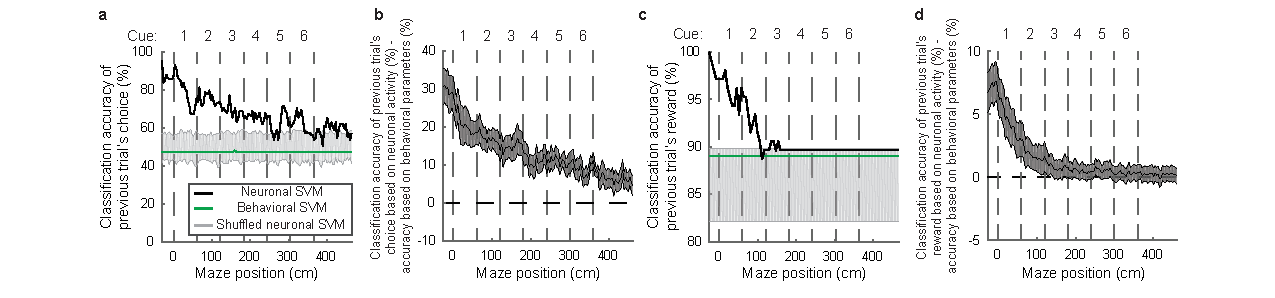
\includegraphics[width=1.2\textwidth,center]{figures/fig_3_13.pdf}
\caption[Contribution of behavioral variability to classification of the previous trial's outcome.]
{\textbf{Contribution of behavioral variability to classification of the previous trial's outcome. a,} Comparison of a neuronal activity-based SVM (black), behavioral parameter-based SVM (green), and the 99\% confidence interval of a neuronal activity-based SVM with shuffled labels (gray) for the previous trial's choice for a single dataset. The behavioral parameter-based SVM could not discriminate the previous trial's choice. Classifiers were trained to distinguish the mouse's choice on the previous trial independently at each bin in the current trial. 
%
\textbf{b,} Difference between the classification accuracy of the neuronal activity-based SVM and the behavioral parameter-based SVM for the previous trial's choice. Error bars represent mean $\pm$ s.e.m. across datasets. 
%
\textbf{c-d,} Same as in (\textbf{a-b}), but with classifiers for whether or not the previous trial was rewarded.
\label{fig:3_13}}
\end{figure}

%FIGURE 3_14
\begin{figure}
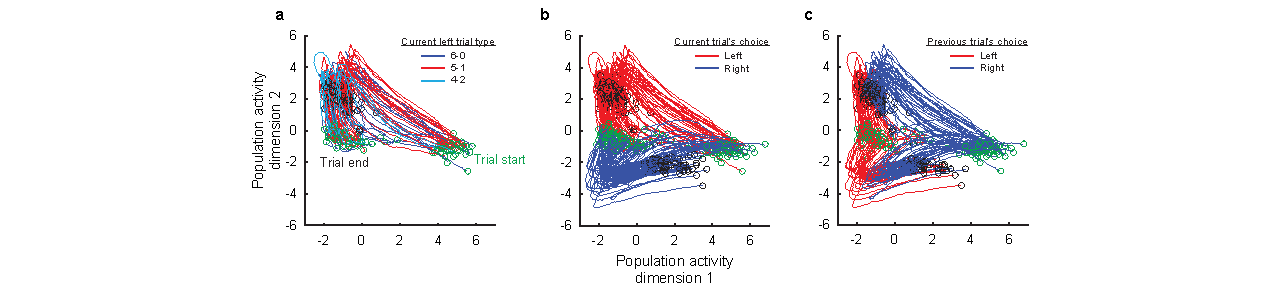
\includegraphics[width=1.5\textwidth,center]{figures/fig_3_14.pdf}
\caption[Visualizations of trial trajectories.]
{\textbf{Visualizations of trial trajectories.} Trajectories of correct trials colored by the current trial type (\textbf{a}), the current trial's choice (\textbf{b}), and the previous trial's choice (\textbf{c}). Trials with the same choice but different trial types were highly overlapping (\textbf{a}), while trials with different choices were highly different (\textbf{b}). Much of the variance within a choice could be explained by the outcome of the previous trial (\textbf{c}). Green and black circles mark the trial start and trial end, respectively. For visualization purposes, the dimensionality of the data was reduced using factor analysis. 
\label{fig:3_14}}
\end{figure}

\subsection{A novel model for evidence accumulation based on history-dependent dynamics} \label{sec:chap3_ev_accum}

Our analyses to this point have focused in large part on comparisons between trials of a single type, but the features identified in these analyses have direct implications for evidence accumulation. We have shown that activity patterns in the PPC partially define the set of possible future activity patterns over seconds (Figure \ref{fig:3_9}). Events that help to establish a new activity pattern will therefore influence the transition probabilities to future activity patterns, creating a short-term memory of the event, as we have shown for choices and reward outcomes across trials (Figure \ref{fig:3_12}). In this framework, we can consider how evidence accumulation might occur. In response to the first evidence cue, the network activity pattern would change based on the type of the evidence cue (left or right cue) and the set of activity pattern transition probabilities at the time of the cue. In response to the second evidence cue, the activity pattern would once again change based on the type of the evidence cue and the set of transition probabilities associated with the current activity pattern. Because the first evidence cue influenced the activity pattern at the time of the second cue, and thus the transition probabilities, the activity pattern resulting after the second cue would be in part a result of both the first and second cues. This same process would be repeated for each subsequent cue. The resulting activity pattern after all cues would therefore be influenced by each previous cue and thus contain information about each of the previous cues. Because this process cascades, the order of the evidence cues would be important. Each unique cue sequence would therefore result in a unique activity pattern, even for the same net evidence. The accumulated evidence cues would be represented generically as a sequence of inputs. In this case, a single abstract variable for net evidence, in which the same final net evidence converges to the same activity pattern, regardless of the cue sequence, is not expected to be present. Our results and their extension therefore make predictions about population activity during evidence accumulation tasks.

\bigskip
A first prediction is that the population activity pattern should reflect not only the net evidence but also the sequence of evidence cues on a trial independent of net evidence. This prediction implies that different sequences of cues that result in the same net evidence (e.g., left-right-left vs. right-left-left) should generate distinguishable activity patterns (Figure \ref{fig:3_15}e). To test this prediction, we selected trial epochs with the same current cue (e.g., left) and the same net evidence (e.g., 1 left) but with different cue types in the previous epoch, thus isolating effects due to the cue history. Trial epochs that had the same cue type in the previous epoch had significantly higher trial-trial population activity correlations than epochs with different cue types in the previous epoch (p < 10\textsuperscript{-9}, two-sample KS test; Figure \ref{fig:3_15}a). Activity in an epoch could therefore be classified above chance levels based on the type of cue in the previous epoch despite identical current cues and net evidences (classification accuracy: 59.0 $\pm$ 2.2\%, mean $\pm$ s.e.m.; p < 0.001, permutation test with shuffled trial labels). While this difference was highly significant, it was relatively modest in amplitude, suggesting that it only accounted for a small fraction of the total trial-trial variability. The activity difference for distinct evidence sequences could reflect different internal accumulated evidence values due to unequal weighting of early and late cues. However, similar results were obtained when we restricted our analysis to the fifth and sixth cues, which were weighted similarly behaviorally, and when we considered data from a mouse that weighted all cues equally (Figure \ref{fig:2_4}, see mouse marked in red; for both cases: p < 0.05, comparison of pairwise activity correlations for trials with the same or different previous cue, two-sample KS test; Figure \ref{fig:3_5}d). The population activity pattern therefore contained information about the sequence of past evidence cues, independent of net evidence, which is consistent with our findings of long-lasting modifications of dynamics by inputs to the PPC.

\bigskip
Another prediction is that the signal for the sequence of past evidence cues (independent of a signal for net evidence) could underlie evidence accumulation in the population activity. Accumulated evidence would therefore be represented implicitly as a sequence of cues rather than explicitly as a single, abstract value such as net evidence. This prediction suggests that population activity with strong signals for cue histories should also have strong signals for evidence accumulation. Taking advantage of the variability across imaging datasets, we found that our ability to decode the sequence of past cues (given the same net evidence) was strongly correlated with the decoding of net evidence (r = 0.84, p < 0.001; Figure \ref{fig:3_15}b). This result indicates that the cue-driven modifications to activity pattern transition probabilities leading to a cue history signal might also serve as the algorithmic mechanism underlying evidence accumulation. 

%FIGURE 3_15
\begin{FPfigure}
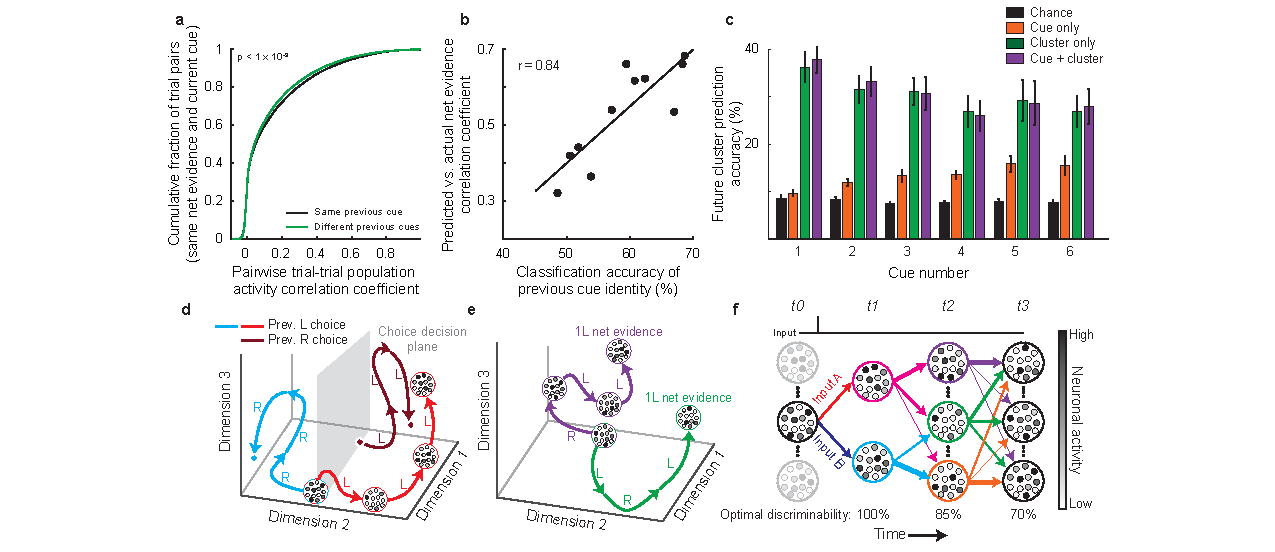
\includegraphics[width=1.3\textwidth,center]{figures/fig_3_15.pdf}
\caption[Analysis of neuronal activity related to evidence accumulation.]
{\textbf{Analysis of neuronal activity related to evidence accumulation. a,} Cumulative distribution of the pairwise trial-trial population activity correlation coefficient for epochs with the same (black) or different (green) previous cues, keeping net evidence, current cue, and epoch constant (e.g., \textit{LRLXXX} vs. \textit{RLLXXX} trials at cue 3) (p < 10\textsuperscript{-9}, two-sample KS test, n = 11 datasets). This analysis tested if neuronal activity at a given epoch contained information about the previous epoch's cue identity, independent of maze epoch, current cue identity, and net evidence. 
%
\textbf{b,} For each dataset, the ability to classify net evidence (correlation coefficient for predicted vs. actual net evidence using SVRs, e.g., as in Figure \ref{fig:3_3}f) was compared with the ability to classify the previous cue's identity (independent of maze epoch, current cue identity, and net evidence, as in (\textbf{a})). Classification of previous cue and net evidence were highly correlated (r = 0.84, p < 0.001, n = 11 datasets), suggesting they might have related mechanisms. 
%
\textbf{c,} For a single trial at a given epoch, the accuracy of predicting the next epoch's cluster identity for that trial based on chance (black), knowledge of the evidence cue only (orange), knowledge of the current cluster identity (green), or both (purple). Error bars represent s.e.m. across 11 datasets. 
%
\textbf{d,} Schematic illustrating that because the population activity depends on both the inputs and the near-past population activity, trials with the the same sequence of cues, but different starting points due to different past events, will take different paths through activity space and ultimately result in distinguishable activity patterns. For example, the red and dark red traces both experience the same same sequence of cues (\textit{LLL}), but start in different locations due to different trial histories, and therefore have different trajectories through activity space. Each large circle with small circles inside of it represents the activity pattern of the network at a given time point, with each small circle indicating the schematized activity of a neuron. Note that activity patterns are transient and change over the course of a trial (see red trajectory). Despite the existence of multiple activity patterns for the same variable (e.g., choice), a decision plane (gray) can be drawn which separates activity patterns according to a given variable. Different decision planes can exist for other variables (e.g., previous trial's choice).
%
\textbf{e,} Schematic depicting that trials with the same starting point and net evidence, but different sequences of cues, will take different paths through activity space, resulting in multiple, distinguishable activity patterns.
%
\textbf{f,} Schematic demonstrating that transient events have a long-lasting impact on network activity by helping to create a new activity pattern with different transition probabilities to future activity patterns. These events therefore influence the set of activity patterns explored over seconds into the future. For example, if the network receives input B, the network transitions to the cyan activity pattern. Trials in the cyan activity pattern at \textit{t1} are most likely to transition to the orange activity pattern at \textit{t2}, less likely to transition to the green activity pattern, and never transition to the purple activity pattern. The identity of the input can therefore be decoded at \textit{t2} as a result of these non-random transitions. Each large circle with small circles inside of it represents a possible activity pattern of the network, with each small circle indicating the schematized activity of a neuron. The thickness of each arrow indicates the probability of a transition between two activity patterns. The transitions between \textit{t0} and \textit{t1} indicate the change in activity due to one of two inputs. Note that the activity patterns both within each time point and across time points are highly different. Because the transition probabilities are probabilistic, memory of the inputs gradually decays as activity patterns diverge, leading to a decrease in the optimal discriminability of inputs A and B over time.  
\label{fig:3_15}}
\end{FPfigure}
%\afterpage{\clearpage}
\clearpage

\bigskip
A final prediction is that if the current activity pattern influences the transition probabilities to future activity patterns, then both the current activity pattern and the type of evidence cue should influence the activity pattern following a new evidence cue. We compared trials with identical net evidence at the same epoch and asked if we could predict the population activity pattern following a new evidence cue (either left or right cue) based on a) the distribution of trials across clusters alone (chance), b) the new cue type alone (cue only), c) the current activity cluster alone (cluster only), and d) both the current activity cluster and the new cue type (cue + cluster) (Methods \ref{methods:clustering_past_future_class}). We performed this analysis in the cluster space to facilitate the analysis of transition probabilities between activity patterns. Based on knowing the new cue’s type, there was an increase in the ability to predict the identity of the next epoch’s activity cluster, indicating that evidence cues triggered changes in population activity (p < 0.001 for cues 2-6; two-sample Student’s t-test). However, the identity of the current activity cluster was more predictive of the next epoch’s activity cluster than was the new cue’s type (p < 0.001 for all cues; two-sample Student’s t-test; Figure \ref{fig:3_15}c). Therefore, although new inputs influenced the future population activity pattern, the past population activity pattern had a larger effect, consistent with a role for the current activity pattern in defining the set of possible future activity patterns.

\section{Acknowledgements}
We thank Selmaan Chettih and Matthias Minderer for developing the cell selection software, Mark Andermann, John Assad, Wolfgang Maass, Ofer Mazor, Stefano Panzeri, and Alexander Trott for helpful discussions, and Bob Datta, Daniel Dombeck, Jan Drugowitsch, Chenghua Gu, and members of the Harvey lab for comments on the manuscript. We also thank the Research Instrumentation Core at Harvard Medical School. This work was supported by a Burroughs-Wellcome Fund Career Award at the Scientific Interface, the Searle Scholars Program, the New York Stem Cell Foundation, the Alfred P. Sloan Research Foundation, a NARSAD Brain and Behavior Research Young Investigator Award, NIH grants from the NIMH (R01MH107620) and NINDS (R01NS089521), and a Stuart H.Q. \& Victoria Quan Fellowship (A.S.M.). C.D.H. is a New York Stem Cell Foundation Robertson Neuroscience Investigator.

\section{Author contributions}
A.S.M. and C.D.H. conceived of the project, designed the experiments and analyses, and wrote the paper. A.S.M. collected and analyzed the data. 


 












